\section{Results}\label{sec:results}

\cref{tab:primary} reports the primary parameters and results. The primary
operating point is \(K=0.736199\), \(k_yd=0.129812\),
\(\omega=7.633372\), and \(f=\SI{16.684}{\giga\hertz}\). The corresponding physical
frequency is above the guided-mode onset and below the retained cutoff.

\begin{table}[htbp]
\centering
\caption{Primary operating parameters and results. The \(A\), \(H\), and
flexoelectric controls are synthetic or explicitly unresolved. The carrier pair
is a primary bulk Hall transfer with stated assumptions.}
\label{tab:primary}
\begin{tabular}{ll}
\toprule
Quantity & Value \\
\midrule
Material & n-type ZnO, \textit{6mm}, \(c\)-axis along \(x_3\) \\
Plate thickness \(d\) & \SI{200}{\nano\metre} \\
Base carrier concentration \(n_0\) & \SI{2e18}{\per\cubic\metre} \\
Electron mobility \(M\) & \SI{0.0175}{\per\volt\per\second} \\
Derived diffusivity \(D\) & \SI{4.55e-4}{\square\metre\per\second} \\
Gradient length \(\ell\) & \SI{50}{\nano\metre} (synthetic) \\
Longitudinal \(K=k_xd\) & 0.736199 \\
Tangential \(k_yd\) & 0.129812 \\
Frequency \(f\) & \SI{16.684}{\giga\hertz} \\
Incident angle & \SI{10.00}{\degree} \\
Reflected angle & \SI{-27.90}{\degree} \\
Edge residual (scaled) & \(3.00\times10^{-15}\) \\
Control-volume power error & \(7.31\times10^{-13}\) \\
Backward self-power at \SI{2}{\micro\metre} (\(H=0\)) & \SI{2.315}{\percent} \\
Backward self-power at \(H/H^*=-0.05\) & \SI{2.286}{\percent} \\
Backward self-power at \(H/H^*=+0.05\) & \SI{2.266}{\percent} \\
\bottomrule
\end{tabular}
\end{table}

\cref{fig:fig01} shows the dispersion, phase, group, and energy velocities. The
energy velocity is computed from \(P_x/W\), not from \(|\omega|/|k|\). In the
low-loss region the three speeds agree; away from the cutoff the carrier loss makes
the energy velocity differ from the phase speed. The power FWHM panel reports the
temporal decay of the primary guided branch.

\begin{figure}[htbp]
\centering
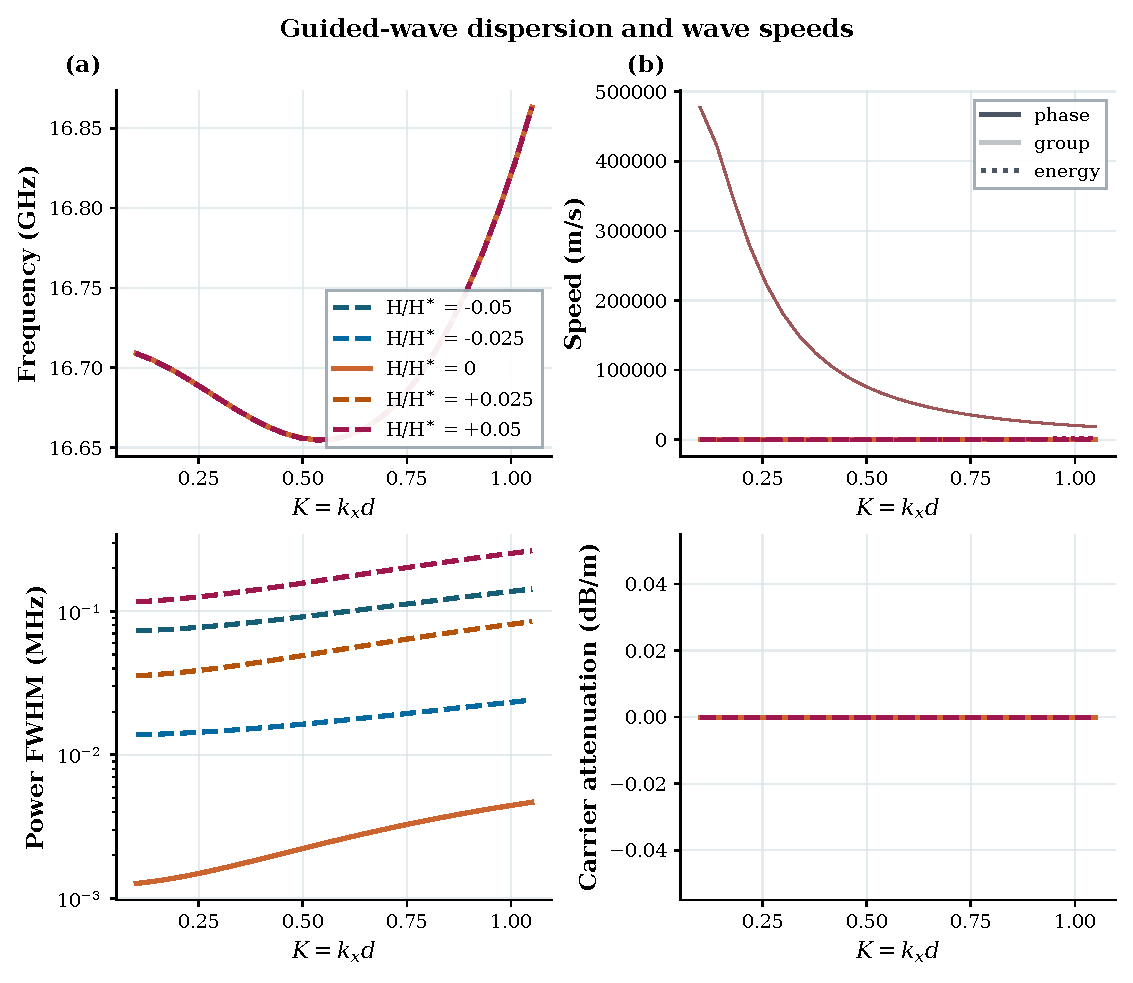
\includegraphics[width=\textwidth]{figures/fig01_dispersion.pdf}
\caption{Dispersion and wave speeds versus \(K=k_xd\) for five normalized
\(H\) values. The energy velocity is thickness-integrated power divided by
thickness-integrated energy. Data:
\texttt{fig01\_dispersion\_velocity\_attenuation.csv}.}
\label{fig:fig01}
\end{figure}

\cref{fig:fig02} shows ordinary material-parameter sensitivity. The baseline
carrier concentration and mobility are highlighted. Increasing \(n_0\) increases
carrier screening and changes the backward self-power; increasing \(M\) changes the
drift--diffusion loss. The reflected self-power remains small and bounded over the
tested ranges.

\begin{figure}[htbp]
\centering
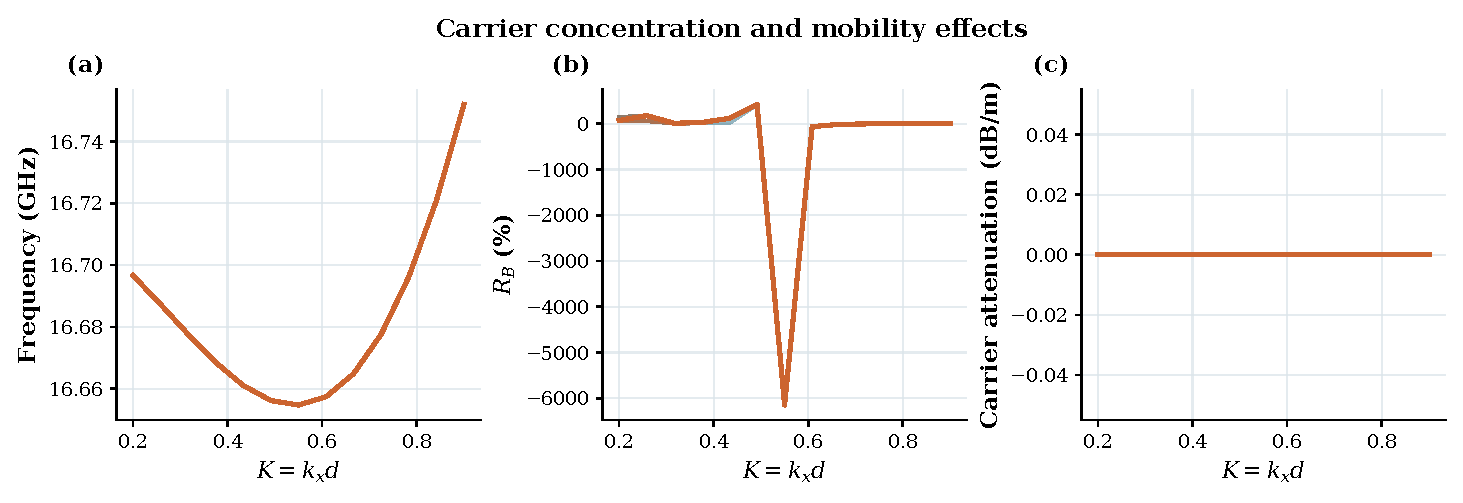
\includegraphics[width=\textwidth]{figures/fig02_material.pdf}
\caption{Carrier concentration and mobility sensitivity. Solid curves are the
baseline values; lighter curves are other tested values. Data:
\texttt{fig02\_material\_parameter\_sweep.csv}.}
\label{fig:fig02}
\end{figure}

\cref{fig:fig03} shows plate thickness and gradient-length sensitivity. The
frequency axis is normalized by \(f_s\), so the displayed frequency is not directly
comparable across thicknesses without rescaling \(f_s\). The cutoff frequency panel
reports the lowest positive-frequency guided branch used as the sweep seed.

\begin{figure}[htbp]
\centering
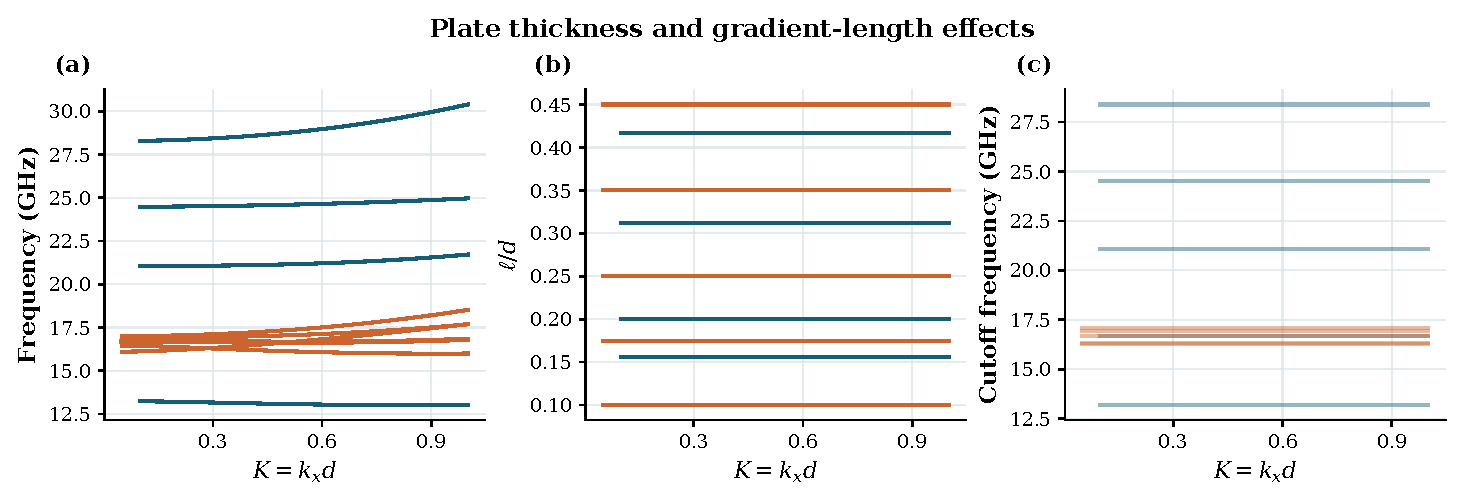
\includegraphics[width=\textwidth]{figures/fig03_geometry.pdf}
\caption{Plate thickness and gradient-length effects. The cutoff frequency is
reported for each tested geometry. Data:
\texttt{fig03\_geometry\_sweep.csv}.}
\label{fig:fig03}
\end{figure}

\cref{fig:fig04} reports the frequency dependence of the isolated backward
transfer. The edge curve removes the reference-plane propagation factor; the
\SI{2}{\micro\metre} curve is the reference-plane isolated self-power; the
\SI{100}{\micro\metre} curve includes the propagation factor. These are isolated
self-flux ratios, not total reflectance.

\begin{figure}[htbp]
\centering
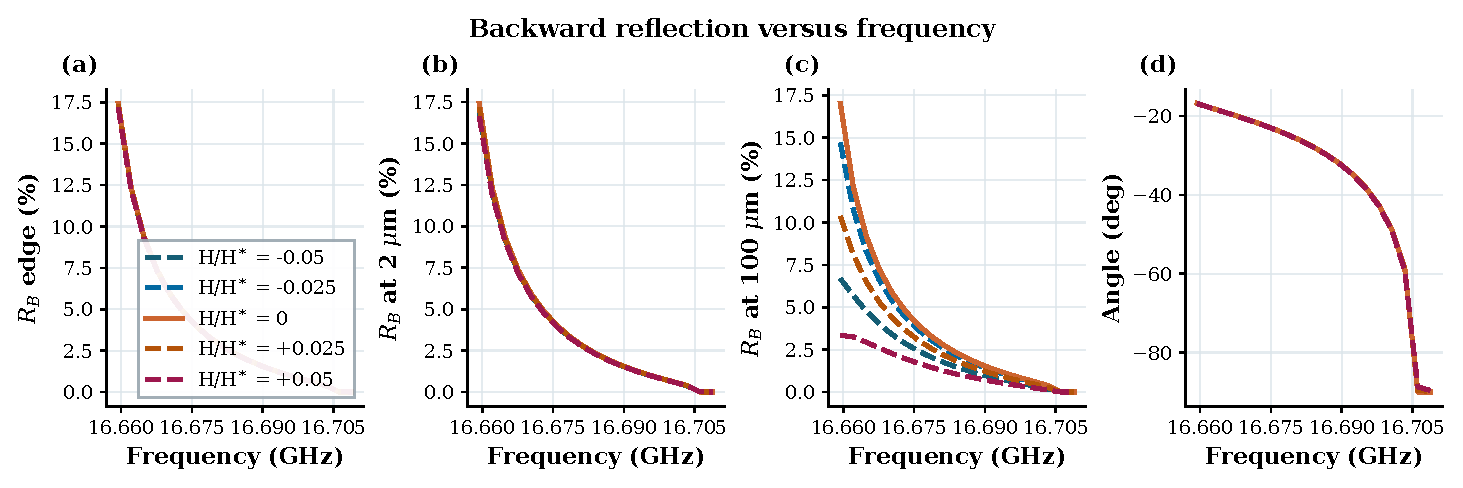
\includegraphics[width=\textwidth]{figures/fig04_frequency.pdf}
\caption{Backward self-power versus frequency. The edge, \SI{2}{\micro\metre}, and
\SI{100}{\micro\metre} panels use different reference planes. Data:
\texttt{fig04\_frequency\_reflection.csv}.}
\label{fig:fig04}
\end{figure}

\cref{fig:fig05} gives the modal self-flux accounting used to classify the
backward channel. The forward self-flux is negligible for the primary case; the
outgoing self-flux is carried by the backward branch. The backward self-flux
fraction is the negative self-flux carried by the backward branch normalized by
the total outgoing self-flux, whereas the isolated reflection metric is the
backward self-power at \SI{2}{\micro\metre} normalized by the incident self-power.
The latter is the quantity reported as \(R_B\).

\begin{figure}[htbp]
\centering
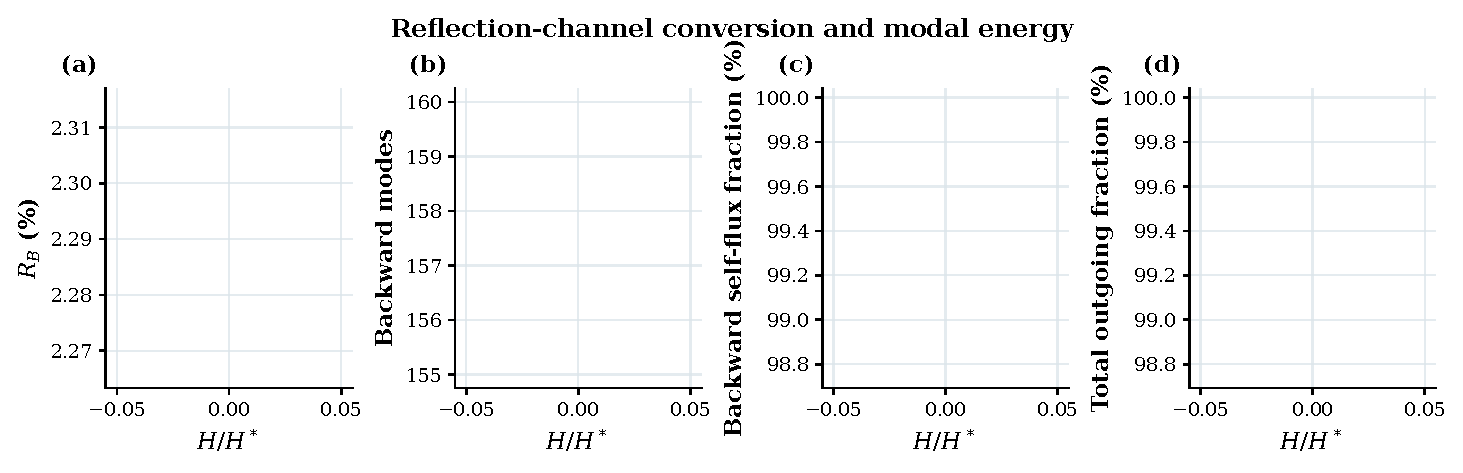
\includegraphics[width=\textwidth]{figures/fig05_channel.pdf}
\caption{Reflection-channel conversion and modal self-flux. The backward fraction
is the negative self-flux carried by the backward branch, normalized by the
incident self-power. Data: \texttt{fig05\_channel\_power.csv}.}
\label{fig:fig05}
\end{figure}

\cref{fig:fig06} shows distance dependence. The isolated backward transfer and the
incident self-flux are separate quantities; at finite distance edge conversion and
propagation attenuation are not generally separable. The incident self-flux grows
with distance because the primary incident branch has positive imaginary \(K\) at
this operating point. This is not a physical gain; it is the mathematical survival
factor of the isolated incident mode.

\begin{figure}[htbp]
\centering
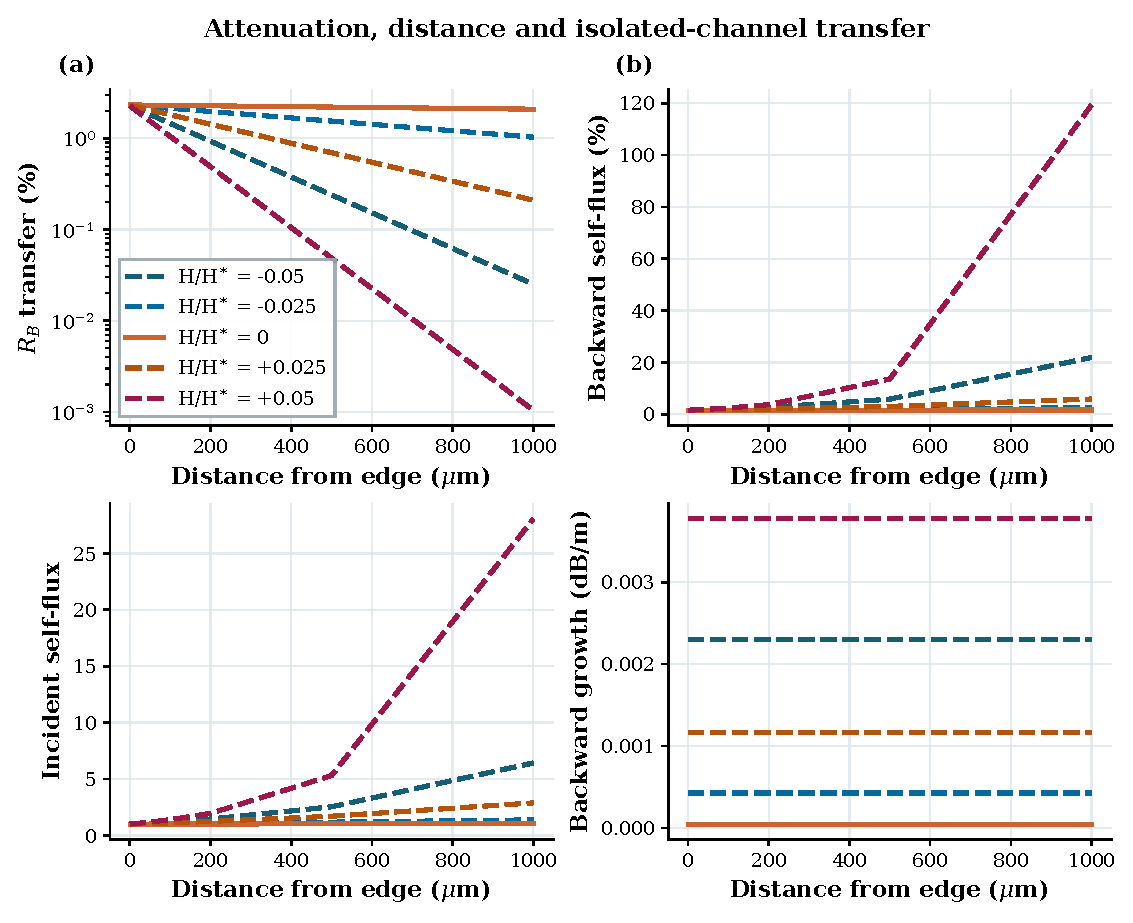
\includegraphics[width=\textwidth]{figures/fig06_attenuation.pdf}
\caption{Distance dependence of isolated backward transfer, backward self-flux,
incident self-flux, and backward growth. Data:
\texttt{fig06\_attenuation\_distance.csv}.}
\label{fig:fig06}
\end{figure}

\cref{fig:fig07} shows \(H/k_y\) coupling sensitivity. The primary tangential
wavenumber is fixed in \cref{tab:primary}; the sweep varies \(k_y\) around that
value and reports the isolated edge transfer. The response is smooth in the tested
range, but no broad-angle negative-reflection sweep is claimed.

\begin{figure}[htbp]
\centering
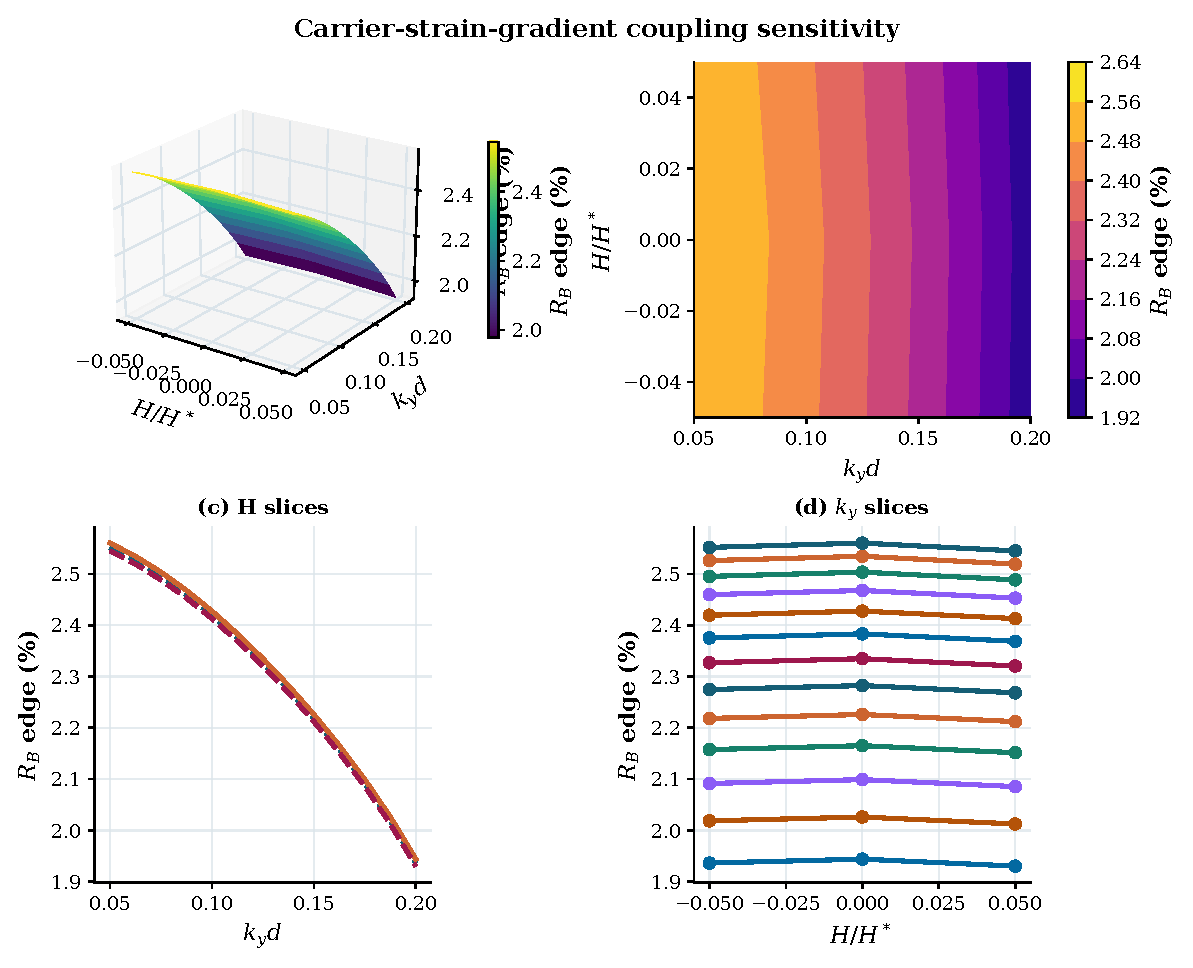
\includegraphics[width=\textwidth]{figures/fig07_coupling.pdf}
\caption{Carrier--strain-gradient coupling sensitivity versus \(H/H^*\) and
\(k_yd\). Data: \texttt{fig07\_coupling\_sensitivity.csv}.}
\label{fig:fig07}
\end{figure}

\cref{fig:fig08} reports boundary-condition sensitivity. Grounded electrical runs
succeed. Open-circuit runs are singular in all tested cases in the present solver;
the figure annotates this failure rather than omitting the open-circuit lines.
No successful open-boundary comparison is claimed.

\begin{figure}[htbp]
\centering
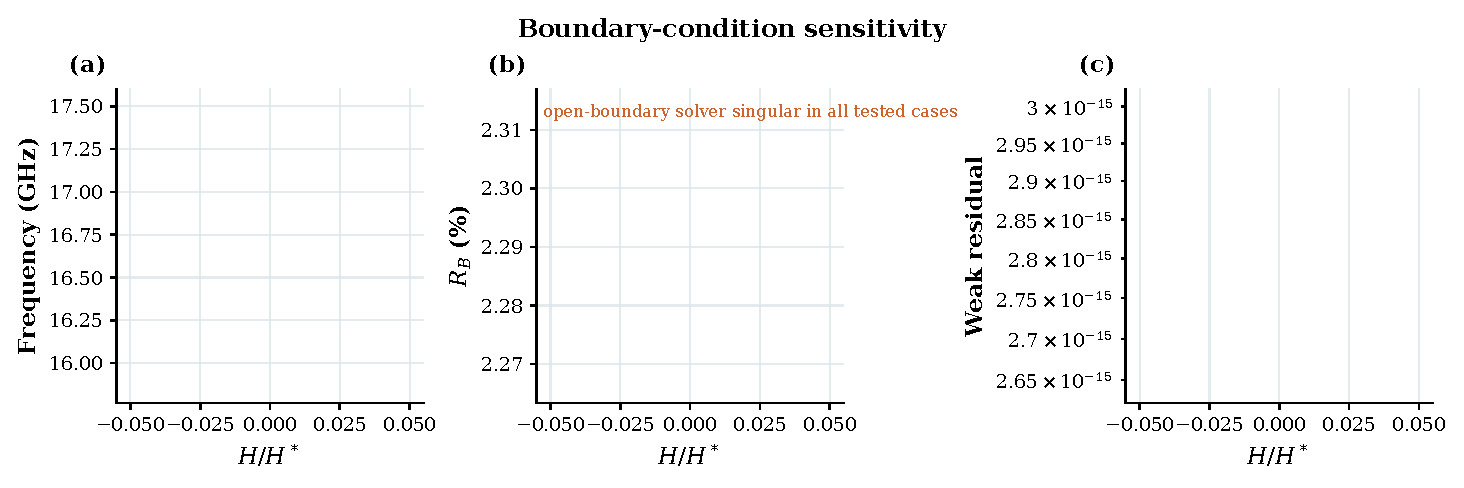
\includegraphics[width=\textwidth]{figures/fig08_boundary.pdf}
\caption{Boundary-condition sensitivity. The open-boundary solver is singular in
all tested cases; the annotation records the failure. Data:
\texttt{fig08\_boundary\_sensitivity.csv}.}
\label{fig:fig08}
\end{figure}

\cref{fig:fig09} shows convergence. The primary backward self-power changes by less
than \(5.9\times10^{-8}\) between Legendre degrees 14 and 26, and the edge residual
remains below \(4\times10^{-15}\). The power-balance error is at the
\(10^{-13}\)--\(10^{-12}\) level and is stable across the tested spectral
resolutions.

\begin{figure}[htbp]
\centering
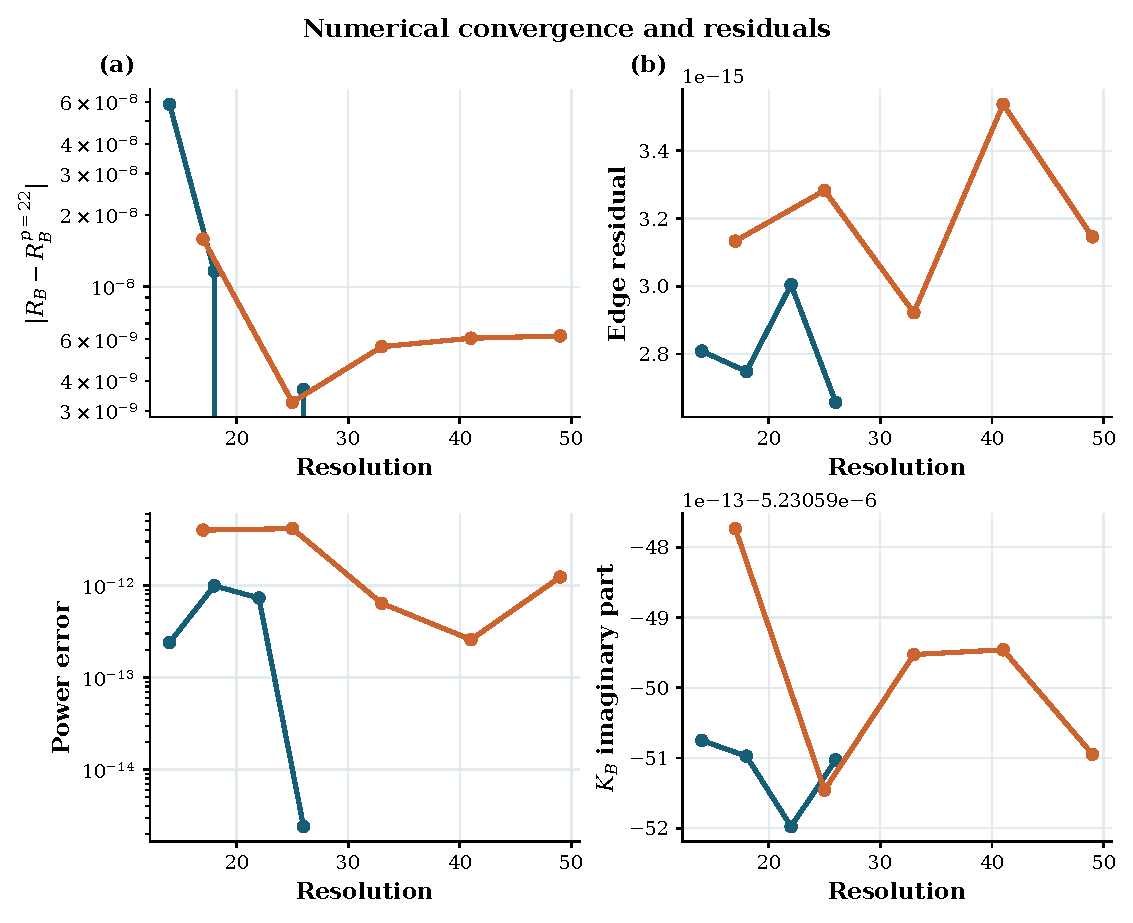
\includegraphics[width=\textwidth]{figures/fig09_validation.pdf}
\caption{Numerical convergence and residuals. Data:
\texttt{fig09\_validation\_convergence.csv}.}
\label{fig:fig09}
\end{figure}

\cref{fig:fig10} shows the solved incident and backward channels near the edge.
The computed backward-channel centroid is approximately zero in \(y\), and the
incident and backward fields remain separated by the edge condition. The field is a
reconstruction from the solved angular spectrum, not an independently measured
field.

\begin{figure}[htbp]
\centering
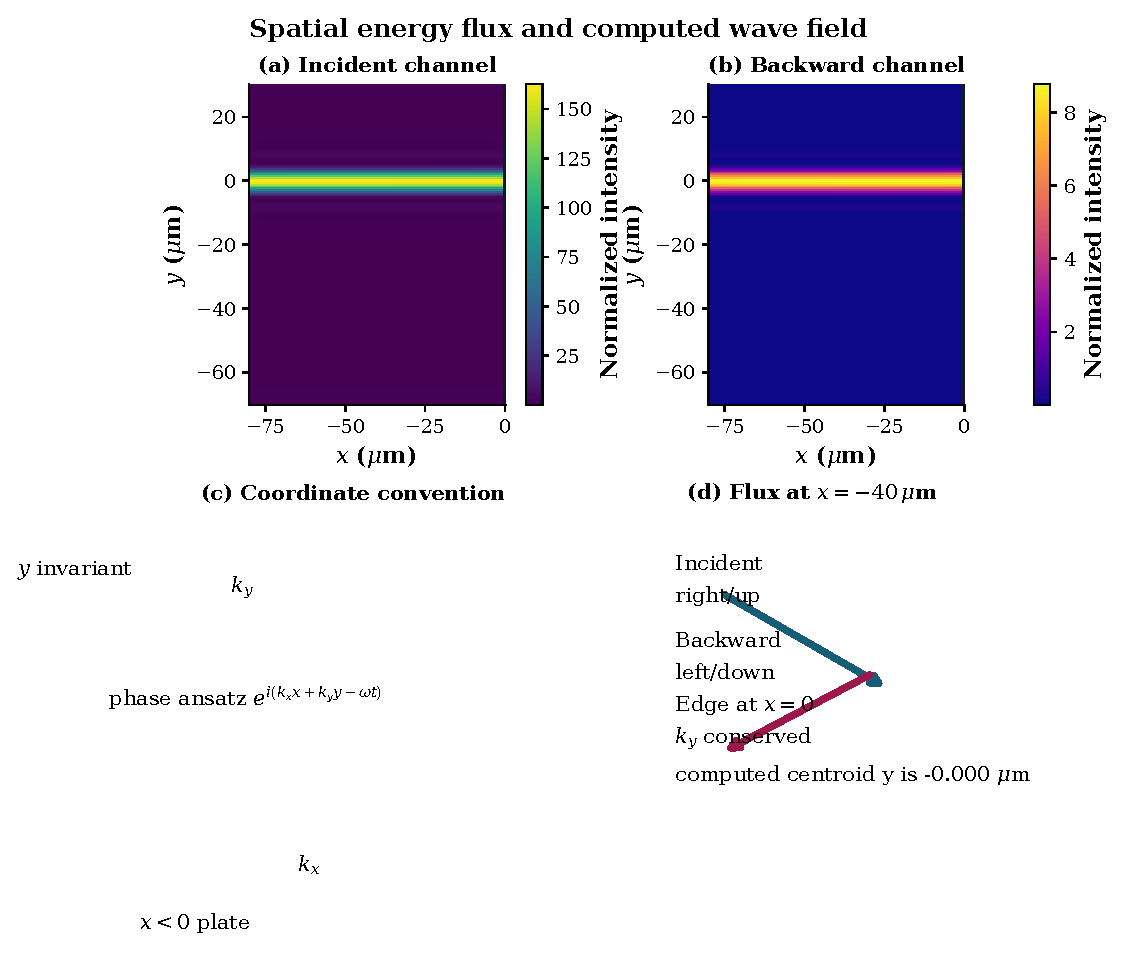
\includegraphics[width=\textwidth]{figures/fig10_field.pdf}
\caption{Solved incident and backward channels near the edge. The coordinate
convention and flux direction are shown in panels (c) and (d). Data:
\texttt{fig10\_field\_metrics.json} and the stored intensity arrays.}
\label{fig:fig10}
\end{figure}
